\section{Reproducing the examples}
\label{app:repro}

All listings in this paper are drawn from the repository's doctested
tutorials, examples, and tests of \pqlang{} 0.8.0.  The commands below
regenerate the artifacts referenced in the text:

\begin{lstlisting}[style=pyqbase, language=bash, caption={Reproduction commands (generation and export have no third-party requirements; native cross-checks require the pinned backend environments).}, label={lst:repro}]
# tutorials and core semantics
python -m unittest discover -s tests/core -v

# gallery: 22 cases, RIR + OriginIR-ext + strict gate set exports
python examples/algorithm_gallery.py            # add --native for backend agreement

# oracle/protocol/QODE/QHAM demonstration programs
python examples/algorithm_contracts.py
python examples/ode_input_models.py             # 11 input-model cases
python examples/input_models.py                 # 14 input-model variants over 4 families
python examples/general_qham.py                 # forced Burgers at order 2
python examples/math_functions.py

# static checks
ruff check src tests examples

# numerical verification campaign (Section 9.3): 475 experiments in 13
# groups, writes machine-readable reports to out/verification/
PYTHONPATH=src <backend-python> tools/run_verification.py
\end{lstlisting}

The native configuration runs the same examples under interpreters
providing \texttt{pysparq} and \texttt{uniqc}; revision pins are recorded in
the repository's backend revision ledger.  The verification campaign
requires both backends: the PySparQ path executes RIR natively through
\texttt{pysparq.rir}, and the OriginIR-ext path uses UnifiedQuantum's
\texttt{Circuit.to\_matrix()}---both contributed as part of this work.

\section{Condensed specifications: RIR and OriginIR-ext}
\label{app:spec}

This appendix makes the paper self-contained at the machine-facing layer
by condensing the two formats of \secref{sec:rir}: the object model and
JSON encoding of RIR~0.3, and the grammar of the OriginIR-ext dialect to
which RIR exports.  The normative artifacts---prose specification, JSON
Schema, serializer, and semantic tests, maintained in lockstep---ship with
the repository; everything below is derived from them, and the JSON and
export listings are verbatim outputs of the repository toolchain.

\subsection{RIR 0.3}
\label{app:spec-rir}

\lstref{lst:rir-grammar} summarizes the abstract grammar.  A program is a
versioned table of modules with one designated entry; a module is a typed
interface (ordered quantum registers, ordered QRAM resources, optional
private \texttt{locals}) plus an ordered instruction body, or no body at
all (open declaration).  Instructions are the seven closed node kinds of
Table~\ref{tab:rir-nodes}; views (\texttt{Ref}) are lists of spans and
never mention physical qubits.

\begin{lstlisting}[style=pyqbase, caption={Abstract grammar of the RIR 0.3 object model.  $X^{*}$ denotes an ordered immutable tuple (possibly empty); \texttt{null} marks an absent body or an unused field; \texttt{name} matches \texttt{[A-Za-z\_][A-Za-z0-9\_]*}.  Shape only: alias-freedom, control protection, call matching, and numeric ranges are enforced by the semantic validator (\secref{sec:rir}).}, label={lst:rir-grammar}]
program     = Program{entry: name; modules: module*;
                    version: "0.1" | "0.2" | "0.3"} .
module      = Module{name: name; registers: register*;
                    resources: resource*; body: instruction* | null;
                    attributes: attribute*; locals: register*} .
register    = Register{name: name; type: regtype} .
regtype     = RegType{kind: "bits" | "uint" | "sint" | "rational";
                    width: integer} .
resource    = Resource{name: name; type: qram} .
qram        = QRAM{address_width: integer; data_width: integer} .
attribute   = (name, (string | integer | float | boolean)) .
span        = Span{register: name; start: integer; width: integer} .
ref         = Ref{parts: span*; type: regtype} .

instruction = primitive | load | store | call | repeat | control | adjoint .
primitive   = Primitive{op: gate-op; operands: ref*;
                    angle: float | null; value: integer | null} .
gate-op     = "h" | "x" | "y" | "z" | "s" | "t" | "rx" | "ry" | "rz"
            | "phase" | "gphase" | "xor" | "swap" | "add_const" .
load        = Load{resource: name; address: ref; data: ref} .
store       = Store{resource: name; address: ref; data: ref} .
call        = Call{module: name; arguments: ref*; resources: name*} .
repeat      = Repeat{count: integer; body: instruction*} .
control     = Control{register: ref; value: integer; body: instruction*} .
adjoint     = Adjoint{body: instruction*} .
\end{lstlisting}

Serialization maps every record to a tagged JSON object whose keys are
exactly the record's fields; tuples become JSON arrays; scalars and null
pass through unchanged.  Whether \texttt{angle} and \texttt{value} are
present is determined by \texttt{op} (unused ones serialize as null).
Decoding is strict---unknown tags or fields, duplicate keys, non-finite
floats, and unknown versions are rejected---and canonical output is UTF-8,
key-sorted, two-space indented, with one trailing newline.  Readers accept
prior versions 0.1 and 0.2, whose modules carry no \texttt{locals} field.
The complete canonical JSON of a minimal closed program---a single
\texttt{h} on a one-bit register, produced by
\texttt{dumps()} on a one-line builder program---is shown in
\lstref{lst:rir-json}.

\begin{lstlisting}[style=pyqjson, caption={Canonical RIR 0.3 JSON (verbatim \texttt{dumps} output) of the module \texttt{h1\{q: Bits(1)\}} containing one \texttt{h}.  All fields are written, including nulls and empty tuples; keys are sorted.}, label={lst:rir-json}]
{
  "entry": "h1",
  "modules": [
    {
      "attributes": [],
      "body": [
        {
          "angle": null,
          "op": "h",
          "operands": [
            {
              "parts": [
                {
                  "register": "q",
                  "start": 0,
                  "tag": "Span",
                  "width": 1
                }
              ],
              "tag": "Ref",
              "type": {
                "kind": "bits",
                "tag": "RegType",
                "width": 1
              }
            }
          ],
          "tag": "Primitive",
          "value": null
        }
      ],
      "locals": [],
      "name": "h1",
      "registers": [
        {
          "name": "q",
          "tag": "Register",
          "type": {
            "kind": "bits",
            "tag": "RegType",
            "width": 1
          }
        }
      ],
      "resources": [],
      "tag": "Module"
    }
  ],
  "tag": "Program",
  "version": "0.3"
}
\end{lstlisting}

\subsection{OriginIR-ext}
\label{app:spec-originir}

OriginIR-ext is the modular textual dialect emitted by
\texttt{export\_originir}.  It is a strict superset of the classical
OriginIR gate vocabulary extended with module definitions, module calls,
QRAM resource declarations, inline control, and symbolic inversion; the
grammar of \emph{emitted} programs is given in \lstref{lst:originir-grammar}.
Every RIR construct has a translation that preserves module definitions
and calls (\secref{sec:rir}, R3/R5): nothing is inlined.

\begin{lstlisting}[style=pyqir, caption={Grammar of the OriginIR-ext dialect as emitted by \texttt{export\_originir}.  \texttt{id} is \texttt{[A-Za-z\_][A-Za-z0-9\_]*}; \texttt{ram} names a declared QRAM resource; definition names consist of the module name and a content hash, making exports deterministic and diff-stable.}, label={lst:originir-grammar}]
program     = qramdecl* qinit creg def* entrycall .
qramdecl    = "QRAMDECL" ram int "," int .
qinit       = "QINIT" int .
creg        = "CREG" int .
def         = "DEF" symbol "(" formal ("," formal)* ")"
              stmt* "ENDDEF" .
formal      = id "[" int "]" .
stmt        = gate | load | store | call | dagger .
gate        = op bit ("," bit)? ("," "(" num ")")? ctrl? .
ctrl        = "controlled_by" "(" bit ("," bit)* ")" .
load        = ram bit ("," bit)* .
store       = "QRAMWRITE" ram bit ("," bit)* .
call        = symbol "(" bit ("," bit)* ")" .
dagger      = "DAGGER" stmt* "ENDDAGGER" .
bit         = id "[" int "]" .
qbit        = "q" "[" int "]" .
entrycall   = symbol "(" qbit ("," qbit)* ")" .
op          = "H" | "X" | "Y" | "Z" | "S" | "T" | "RX" | "RY" | "RZ"
            | "U1" | "CNOT" | "SWAP" .
\end{lstlisting}

The header declares the entry program's QRAM resources
(\texttt{QRAMDECL ram\_\ s a,d}), allocates the total qubit count including
workspace (\texttt{QINIT n}), and fixes the classical register width
(\texttt{CREG 0}: measurement and classical readout remain host-side).
The lowering rules for the RIR surface are:

\begin{itemize}
\item \textbf{Definitions.}  Each module compiles to one \texttt{DEF} per
  required specialization, with formals \texttt{v\_\ s[w]} for the
  interface registers, \texttt{pw\_work[k]} when workspace must be passed
  through to the body or callees, and \texttt{pc\_control[c]} when the
  definition is a control specialization.  Definition names embed a
  content hash, so identical specializations are shared and the export is
  reproducible.
\item \textbf{Control.}  On gates and QRAM loads, control is an inline
  \texttt{controlled\_by (bits)} suffix; control bits testing~0 are
  X-conjugated around the statement.  On module calls, control does not
  fan out per gate: the callee is specialized with \texttt{pc\_control}
  formals and the control bits are passed as ordinary call arguments.
\item \textbf{Adjoint.}  \texttt{DAGGER}~\dots~\texttt{ENDDAGGER} wraps the
  lowered body; the adjoint of a call is the daggered call line.
\item \textbf{Classical memory writes.}  \texttt{Store} lowers to
  \texttt{QRAMWRITE} with address and data bits. Its definite-value
  precondition and prohibition inside controlled or adjoint contexts
  follow the RIR semantics. The current native text-execution paths
  reject runtime writes; text export does not imply backend support.
\item \textbf{Repeat.}  There is no textual repetition construct: a count
  of $n$ compiles to a chain of shared definitions in which the definition
  for $n$ calls the definition for $\lfloor n/2 \rfloor$ twice (plus the
  base once more when $n$ is odd).  The body text is emitted once and the
  listing grows logarithmically in $n$.
\item \textbf{Primitives.}  Broadcast gates fan out per bit;
  \texttt{rx/ry/rz/phase} become \texttt{RX/RY/RZ/U1} with the angle in
  parentheses; \texttt{xor} and \texttt{swap} become per-bit
  \texttt{CNOT}/\texttt{SWAP}; \texttt{add\_const} lowers to a
  multi-controlled-X staircase; \texttt{gphase} anchors a conjugated
  \texttt{U1} pair on the first interface bit (the four-line sandwich
  realizes $e^{i\theta}I$ on the whole register).
\item \textbf{Entry.}  The single top-level call binds the entry module to
  the physical bits \texttt{q[0..n-1]} in register order followed by
  workspace---the only place physical qubit indices appear, and they
  appear in text, not in the RIR.
\end{itemize}

\lstref{lst:originir-lowered} shows a complete export exercising the
non-trivial rules: a controlled constant addition (the
\texttt{controlled\_by} staircase), a \texttt{Repeat} of five rotations
(the two-definitions-plus-base chain of the shared-module rule), and a
symbolic adjoint.

\begin{lstlisting}[style=pyqir, caption={OriginIR-ext export (verbatim \texttt{export\_originir} output) of the module \texttt{demo\{word: UInt(4), flag: Bits(1)\}} that applies \texttt{h} to \texttt{word}, adds the constant 3 under control of \texttt{flag}, repeats \texttt{rz(0.5)} on \texttt{word[0]} five times, and adjoints \texttt{x} on \texttt{word[1]}.  The three \texttt{m\_demo\_*} definitions are the logarithmic chain for count 5; note the propagated \texttt{v\_flag[0]} argument replacing per-gate controls inside called modules.}, label={lst:originir-lowered}]
QINIT 5
CREG 0
DEF m_demo_f1a56b9995841efc84b9e7fa(v_word[4], v_flag[1])
RZ v_word[0], (0.5)
ENDDEF
DEF m_demo_28de1671d87f7f6741cc1b1e(v_word[4], v_flag[1])
m_demo_f1a56b9995841efc84b9e7fa(v_word[0], v_word[1], v_word[2], v_word[3], v_flag[0])
m_demo_f1a56b9995841efc84b9e7fa(v_word[0], v_word[1], v_word[2], v_word[3], v_flag[0])
ENDDEF
DEF m_demo_69bd809b9442abd5102ed4d4(v_word[4], v_flag[1])
m_demo_28de1671d87f7f6741cc1b1e(v_word[0], v_word[1], v_word[2], v_word[3], v_flag[0])
m_demo_28de1671d87f7f6741cc1b1e(v_word[0], v_word[1], v_word[2], v_word[3], v_flag[0])
m_demo_f1a56b9995841efc84b9e7fa(v_word[0], v_word[1], v_word[2], v_word[3], v_flag[0])
ENDDEF
DEF m_demo_5470c8daec78cb3d0a711209(v_word[4], v_flag[1])
H v_word[0]
H v_word[1]
H v_word[2]
H v_word[3]
X v_word[3] controlled_by (v_flag[0], v_word[0], v_word[1], v_word[2])
X v_word[2] controlled_by (v_flag[0], v_word[0], v_word[1])
X v_word[1] controlled_by (v_flag[0], v_word[0])
X v_word[0] controlled_by (v_flag[0])
X v_word[3] controlled_by (v_flag[0], v_word[1], v_word[2])
X v_word[2] controlled_by (v_flag[0], v_word[1])
X v_word[1] controlled_by (v_flag[0])
m_demo_69bd809b9442abd5102ed4d4(v_word[0], v_word[1], v_word[2], v_word[3], v_flag[0])
DAGGER
X v_word[1]
ENDDAGGER
ENDDEF
m_demo_5470c8daec78cb3d0a711209(q[0], q[1], q[2], q[3], q[4])
\end{lstlisting}

A second backend pass lowers the same artifact further to the strict
\{\textsc{toffoli}, $U_3$, \textsc{cz}\} gate set with ancilla pooling
(\secref{sec:architecture}); it operates on the OriginIR-ext text and,
like every downstream consumer, never feeds back into the RIR.


\section{Four solver families in code}
\label{app:families}

This appendix shows complete input programs---drawn verbatim from the
repository's doctested examples---for four representative solver
territories of \secref{sec:ode}: three of the six ODE families
(Carleman, LCHS, and the contour family CBMD) and the QHAM PDE path; the
remaining families (Schr\"odingerization, Euler--QLSS history systems,
and Taylor kernels) follow the same pattern with their own generators.
Comments are translated from Chinese, and artifact bookkeeping is elided
at the marked points.  The point of
interest is not the numerics but what stays \emph{open} and what is
\emph{swappable} in each family: every listing contains at least one
\texttt{abstract\_*} declaration that the same program could bind
differently, and every solver entry accepts its kernel configuration as an
argument (R1, R2, R5).

\subsection{QHAM: from a symbolic PDE to a solver-ready input model}
\label{app:qham}

\subsubsection{Background, method, and input models}
\label{app:qham-method}

\paragraph{The method, tutorially.}
Two ideas anchor this family, and the listing is best read as their
composition.  The first is the homotopy analysis method
(HAM)~\cite{liao2003beyond,liao2012homotopy}: to solve a nonlinear
equation $N[u]=0$, do not linearize around a small parameter (there may
not be one); instead \emph{deform} a solvable linear problem into the
target along an artificial embedding parameter $q\in[0,1]$,
\[
H(v,q) \;=\; (1-q)\,\bigl(L[v]-f\bigr) \;+\; q\,N[v] \;=\; 0 ,
\]
where $L$ is a chosen linear base operator.  At $q=0$ the problem is
linear; at $q=1$ it is the target.  Expanding the solution as a power
series in $q$ and truncating at order $m$ yields a \emph{hierarchy of
linear problems} whose solvability and convergence are governed by an
auxiliary parameter (the $\eta=-0.4$ of the listing) that the analyst
chooses freely---this freedom is what distinguishes HAM from perturbation
expansions.  For a polynomial PDE, the order-$m$ truncation collapses the
hierarchy into a single \emph{lifted linear generator} whose coefficients
are polynomial functions of the state; a quantum computer never touches
the nonlinearity directly, only block-encodings of these coefficient
tensors.

The second idea is the solver the listing hands the lifted problem to:
Schr\"odingerization~\cite{jin2024schrodingerization,hu2024schrocircuits}.
A linear evolution $u'=Gu$ with $G=H_1+iH_2$ is not unitary, so it cannot
be simulated directly; the trick is to embed the state in a space with
one extra \emph{momentum} coordinate $p$, prepare the warped initial
state $e^{-|p|}\otimes u_0$, and Fourier-transform along $p$.  In the
transformed space the dynamics become an honest Hamiltonian evolution
under the lifted generator $K'=-P\otimes H_1 - I\otimes H_2$ (our
convention after the sign repair of \secref{sec:numverify}), which
ordinary Hamiltonian simulation handles; the physical solution is
recovered from a single Fourier channel, up to the known factor
$e^{p_{\mathrm{sel}}}$---the warp $e^{-|p|}$ decays exactly at the rate
the non-unitary part $H_1$ demands, which is why one channel suffices.

\paragraph{What the input models represent.}
The listing states the \emph{mathematics} and defers the \emph{physics
ownership}.  A \texttt{PolynomialPDE} over \texttt{Field} expressions is
the problem itself, entered symbolically; the forcing term
\texttt{Known("forcing")} is \emph{data by name}---the program says
``some table with this identity exists'' without deciding whether it will
be baked into gates, served from a QRAM, or supplied by a collaborator.
\texttt{structured\_fd\_bindings} then makes the one concrete decision
the tutorial level requires---a finite-difference discretization---and
returns \emph{stencil-structured ports}: gate-level realizations of the
stencil operators plus a norm-preserving lifted initial state.  The
product \texttt{qode\_input} is an open QODE input model; the solver is
selected by name at the far end of the pipeline with its approximation
kernel injected (\texttt{taylor\_hamiltonian}, degree 1 here).  Every
binding above is replaceable without touching the problem statement,
which is the R1/R2 discipline the appendix exists to exhibit.

\paragraph{Flow of the listing.}
\begin{enumerate}
\item enter the PDE symbolically (\texttt{PolynomialPDE.from\_equations},
  forcing as \texttt{Known} data);
\item fix the homotopy truncation order $m{=}2$ and parameter
  $\eta{=}{-}0.4$ in a lazily computed \texttt{QHAMPlan} (a row-rule plan
  that never materializes tensor blocks, R5);
\item discretize (\texttt{structured\_fd\_bindings}) into stencil ports
  and the lifted initial state;
\item emit the open input model \texttt{qham\_input\_model}; and
\item solve: \texttt{linear\_qode("schrodingerization",} $\ldots)$ at
  $t=0.01$, with recovery-interval validation recorded pending.
\end{enumerate}

\lstref{lst:qham} is the repository's forced-Burgers example
(\texttt{examples/general\_qham.py}) in full.  The equation is entered
\emph{symbolically}---a \texttt{PolynomialPDE} over a \texttt{Field}
expression, with the forcing term declared as named data
(\texttt{Known("forcing")}) rather than a baked-in array.  The homotopy
plan fixes the linearization order ($m=2$) and the homotopy parameter
($\eta=-0.4$); the structured finite-difference bindings carry the
stencil-structured ports and the lifted initial state.  The result,
\texttt{qode\_input}, is an open QODE input model: it can be handed to any
solver family, and the physically owned pieces (coefficient block-encodings,
forcing data) remain bindable separately.

\begin{lstlisting}[style=pyqpython, caption={QHAM end to end: symbolic polynomial PDE, homotopy-analysis plan, structured discretization, and a solver handed in from outside (verbatim from the doctested example \texttt{examples/general\_qham.py}; comments translated).}, label={lst:qham}]
from functools import partial

from pyqecclang.algorithms.hamiltonian import taylor_hamiltonian
from pyqecclang.algorithms.ode import linear_qode
from pyqecclang.applications.qham import (
    Discretization,
    Field,
    Grid,
    Known,
    PolynomialPDE,
    QHAMPlan,
    qham_input_model,
    structured_fd_bindings,
)

u = Field("u")
pde = PolynomialPDE.from_equations(
    {"u": 0.1 * u.d("x", 2) - u * u.d("x") + Known("forcing")},
    label="forced_burgers",
)
plan = QHAMPlan(pde, order=2)
grid = Grid(("x",), (4,), (1.0,), boundary="periodic")
space = Discretization(pde, grid, {"forcing": [0.05, 0, -0.05, 0]})
initial = space.encode_fields({"u": [0.1, 0.2, 0, -0.1]})
bindings = structured_fd_bindings(space, initial)
qode_input = qham_input_model(plan, bindings, eta=-0.4)

# Schrodingerization accepts a general generator; recovery-interval and
# time-approximation validation remains a pending item.
solver = linear_qode(
    "schrodingerization", hamiltonian_function=partial(taylor_hamiltonian, degree=1)
)
solution = qode_input.solve(solver, 0.01)
\end{lstlisting}

\subsubsection{Line-by-line walkthrough}
\label{app:qham-lines}

The listing above is the complete user-side program; this subsection walks
through it line by line and states, for each line, what the library
actually constructs.

\begin{itemize}
\item \texttt{from functools import partial} --- standard-library helper;
  used at the solver line to \emph{inject} the Hamiltonian-simulation kernel
  as a partially applied argument.  The kernel is a value, not a global
  choice (R8).
\item \texttt{from pyqecclang.algorithms.hamiltonian import
  taylor\_hamiltonian} --- the default Hermitian-simulation kernel family;
  its \texttt{degree} argument controls the truncation order of the Taylor
  series.
\item \texttt{from pyqecclang.algorithms.ode import linear\_qode} --- the
  uniform solver front: the family is selected by a name string
  (\texttt{"lchs"}, \texttt{"schrodingerization"}, \texttt{"cbmd"},
  \dots) and the kernel by an ordinary argument.
\item \texttt{from pyqecclang.applications.qham import \dots} --- the QHAM
  application layer: the symbolic PDE surface (\texttt{Field},
  \texttt{Known}, \texttt{PolynomialPDE}), the discretization objects
  (\texttt{Grid}, \texttt{Discretization}), the linearization plan
  (\texttt{QHAMPlan}), the structured port compiler
  (\texttt{structured\_fd\_bindings}), and the input-model assembler
  (\texttt{qham\_input\_model}).
\item \texttt{u = Field("u")} --- creates a one-atom symbolic expression.
  Overloaded arithmetic (\texttt{+}, \texttt{*}, \texttt{.d(axis, order)})
  builds normalized polynomial terms; unknown fields and \texttt{Known}
  data are \emph{different atom kinds}, so ``who owns this coefficient''
  is visible in the term structure itself rather than in a comment.
\item \texttt{pde = PolynomialPDE.from\_equations(\{"u": 0.1*u.d("x", 2) -
  u*u.d("x") + Known("forcing")\}, label="forced\_burgers")} --- validates
  and freezes the equation into immutable term tuples.  The right-hand side
  is read as: linear diffusion $0.1\,\partial_x^2 u$, quadratic convection
  $-u\,\partial_x u$, and a named forcing table.
  \texttt{from\_equations} also derives the \emph{port decomposition}:
  single-field linear terms form port $L$, pure-data terms form port $F$,
  and each arity-$\ge 2$ term becomes its own port $B_i$---exactly the
  decomposition the stencil layer implements later.
\item \texttt{plan = QHAMPlan(pde, order=2)} --- the homotopy truncation
  plan.  It stores no matrices; it is a row-rule object that lazily answers
  which lifted blocks exist (closure rule $(D{-}1)\sum \text{orders} +
  \text{rank} \le (D{-}1)m{+}1$, here grade $D{-}1{=}1$, max tensor rank
  $3$), how blocks couple (\texttt{row\_terms}), and where each block sits
  in the lifted register (\texttt{offset}).  Homotopy weights are symbolic
  formulas in $\eta$---$1{-}(1{+}\eta)^p$ on physical rows,
  $-\eta(1{+}\eta)^p$ on correction rows---evaluated only when the
  generator is assembled.
\item \texttt{grid = Grid(("x",), (4,), (1.0,), boundary="periodic")} ---
  one axis, four points, unit spacing, periodic wrap.  The grid maps
  derivatives to centered finite-difference stencils applied with periodic
  wrapping; its address width (2 bits here) becomes the spatial register
  width.
\item \texttt{space = Discretization(pde, grid, \{"forcing": [.05, 0,
  -.05, 0]\})} --- joins PDE and grid.  The constructor checks that the
  axes match and that \emph{every} \texttt{Known} name carries data
  covering the grid---the forcing table named in the equation is bound to
  concrete numbers here, at the moment the host owns it.
\item \texttt{initial = space.encode\_fields(\{"u": [.1, .2, 0, -.1]\})}
  --- embeds the four-point initial profile into the full amplitude vector
  of the discretized register (component-wise slicing; all field
  components required).
\item \texttt{bindings = structured\_fd\_bindings(space, initial)} --- the
  only line that compiles gates.  For every PDE port, each term becomes a
  block-encoding: derivative factors are periodic-shift LCUs on the
  spatial register; known-coefficient factors become either scaled
  identities or a controlled-$R_y$ diagonal multiplier (a small database);
  arity-$\ge 2$ terms are contracted in a single builder module whose
  target register stacks one copy of the grid register per operand plus
  component bits, with signal qubits carrying the LCU branches.  Ports are
  then summed by LCU, the initial state becomes a gate state preparation,
  and its Euclidean norm is recorded.  The result is a
  \texttt{QHAMBindings} object---ports plus initial state plus norm, with
  no solver attached.
\item \texttt{qode\_input = qham\_input\_model(plan, bindings, eta=-0.4)}
  --- assembles the lifted \emph{linear} problem.  The generator walk
  enumerates the plan's blocks and couplings, evaluates the homotopy
  weights at $\eta{=}{-}0.4$, places each port into the lifted register at
  the block offsets the plan computes, and LCUs everything into one
  generator block-encoding.  The lifted initial state prepares the physical
  block from the normalized field and the tensor blocks from powers of the
  recorded norm, carrying $\log\lVert u_0\rVert$ as provenance.  What
  returns is a \texttt{QHAMInputModel}: generator, initial state, and the
  two adapters \texttt{solve} and \texttt{dissipative\_shift}.
\item A call to \texttt{linear\_qode} selects Schr\"odingerization and
  supplies a degree-one Taylor kernel through its Hamiltonian-function
  argument. This picks the solver family and injects the branch-simulation kernel by
  argument; nothing in the assembled problem knows which kernel will
  simulate the Hermitian branches.  Swapping this line for another family
  or kernel changes nothing above it.
\item \texttt{solution = qode\_input.solve(solver, 0.01)} --- executes the
  model at $t{=}0.01$: the solver consumes the generator block-encoding and
  the lifted initial state, \texttt{solve} post-selects the physical block
  of the output register, and the returned state oracle is annotated with
  the full plan JSON, the initial-norm bookkeeping, and the recorded
  pending items (recovery-window and time-approximation validation)---R6
  provenance attached to the artifact, not to the paper.
\end{itemize}

The pattern to notice: lines~1--12 are \emph{data and plans} (symbolic
equations, truncation order, grid, tables, initial profile); exactly one
line compiles circuits; one line assembles the lifted linear problem; and
the solver is a swappable argument on the final line.  Every object
crossing a line boundary satisfies a protocol, which is what makes the
same problem object consumable by LCHS, Schr\"odingerization, or CBMD
without change.

\subsection{Carleman: nonlinear lift with a swappable linear solver}
\label{app:carleman}

\subsubsection{Background, method, and input models}
\label{app:carleman-method}

\paragraph{The method, tutorially.}
Carleman linearization trades nonlinearity for
dimension~\cite{liu2021pnas,liu2023carleman}.  For a polynomial ODE
$u'=F(u)=\sum_p F_p\,u^{\otimes(p-1)}\!\cdot u$ on $d$-dimensional state
space, form the \emph{level space} whose $j$-th block is the rank-$j$
tensor power $z_j = u^{\otimes j}$.  Differentiating each level couples it
only to \emph{higher} levels, $z_j' = \sum_{p\ge 1} F_p\, z_{j+p-1}$: the
nonlinear dynamics induce a genuinely linear---but infinite---system on
level space.  Truncating at cutoff $K$ (levels above $K$ discarded)
yields a finite linear system $G_K$ of dimension $O(dK)$, solvable by any
linear solver; the physical state is the level-one block.  The error is
where physics enters: for \emph{strongly dissipative} systems the
reaction terms are too weak to pump amplitude into high levels, and the
truncation tail decays exponentially in $K$---the main result of the
Carleman line is that in this regime the quantum cost is polynomial in
$\log(1/\varepsilon)$ and $d$, with no dependence on integration
time~\cite{liu2021pnas,liu2023carleman}.  Dissipativity is thus a
quantitative promise about the problem, exactly the kind of thing R6
wants carried with the code.

\paragraph{What the input models represent.}
The listing makes the trade visible at the interface.  Each polynomial
coefficient $F_p$ of the lifted generator is declared as an \emph{open}
block-encoding slot \texttt{BurgersF$p$}: the slot says ``this is a
block-encoding of the order-$p$ coefficient tensor, width and scale
factor $\alpha$ as recorded,'' while the binding dict supplies the
concrete operation produced by the stencil ports.  Swap the
discretization, rebind five names---problem assembly is untouched.  The
lifted initial state is likewise an open slot
(\texttt{BurgersInitial}) with the host tracking \texttt{initial\_norm}:
because level $j$ has norm $\lVert u_0\rVert^{\,j}$, the norm is a real
promise about the lifted problem, not a typing detail.  Finally, the
\emph{linear solver is an argument}: \texttt{carleman\_qode(linear\_solver=...,
cutoff=2)} lands in exactly the same solver position as every other
family---the listing solves the same Burgers problem twice, through
Schr\"odingerization and through norm-shifted LCHS, to show that the
Carleman pipeline is solver-agnostic by construction.

\paragraph{Flow of the listing.}
\begin{enumerate}
\item discretize the nonlinear PDE and expose each $F_p$ as the open slot
  \texttt{BurgersF$p$} (with width/$\alpha$ recorded at declaration);
\item declare the lifted initial state open
  (\texttt{BurgersInitial}), the host tracking the initial norm;
\item assemble the truncated generator at \texttt{cutoff=2} over level
  space; and
\item solve the lifted \emph{linear} problem with the injected
  \texttt{linear\_solver}, then read the level-one block; the truncation
  tail is a recorded pending item.
\end{enumerate}

\lstref{lst:carleman} (case~6 of \texttt{examples/ode\_input\_models.py})
runs the inviscid Burgers equation through the Carleman pipeline.  Each
polynomial coefficient $F_p$ of the lifted generator is declared as an
\emph{open} block-encoding slot (\texttt{BurgersF$p$}) and bound to the
operation produced by the stencil ports, so the discretization could be
replaced without touching the problem assembly.  The lifted problem is a
\texttt{PolynomialODE}; the solver,
\texttt{carleman\_qode(linear\_solver=..., cutoff=2)}, receives the linear
solver as an argument, and the loop solves the \emph{same} nonlinear
problem twice---once through Schr\"odingerization and once through
norm-shifted LCHS---which is exactly the ``Carleman lands in the same
linear-solver position'' claim of \secref{sec:ode-solvers}.

\begin{lstlisting}[style=pyqpython, caption={Carleman lift of Burgers: open coefficient block-encodings, an open lifted initial state, and a linear solver injected per call (verbatim from case~6 of \texttt{examples/ode\_input\_models.py}; comments translated, artifact serialization elided).}, label={lst:carleman}]
u = Field("u")
pde = PolynomialPDE.from_equations({"u": 0.1 * u.d("x", 2) - u * u.d("x")})
space = Discretization(pde, grid)
ports = structured_fd_bindings(space, space.encode_fields({"u": [0.1, 0.2, 0, -0.1]}))
concrete = polynomial_from_bindings(ports)
coefficient_slots, bindings = [], {}
for order, coefficient in concrete.coefficients:
    name = "BurgersF" + str(order)
    slot = abstract_block_encoding(
        name, coefficient.width, coefficient.signal_qubits, coefficient.alpha
    )
    coefficient_slots.append((order, slot))
    bindings[name] = coefficient.operation
initial_slot = abstract_state_prep(
    "BurgersInitial", concrete.width, concrete.initial.work_width
)
bindings["BurgersInitial"] = concrete.initial.operation
problem = PolynomialODE(
    concrete.width, tuple(coefficient_slots), initial_slot, concrete.initial_norm
)
recovery = {}
for method, solver in (
    ("schrodingerization", schrodinger),
    ("shifted_lchs", shifted_solver(lchs, recovery)),
):
    nonlinear_solver = partial(carleman_qode, linear_solver=solver, cutoff=2)
    state = qpde_solver(nonlinear_solver)(PDEInput(problem, "burgers"), time)
\end{lstlisting}

\subsection{LCHS: one open program, two data-path realizations}
\label{app:lchs}

\subsubsection{Background, method, and input models}
\label{app:lchs-method}

\paragraph{The method, tutorially.}
The obstacle LCHS removes is non-Hermiticity: $e^{Gt}$ with
$G=H_1+iH_2$ is not unitary, so none of the Hamiltonian-simulation
machinery applies.  The observation is that for a \emph{dissipative}
generator ($H_1$ negative semidefinite), the decaying exponential has a
Cauchy-type integral representation whose branches are unitary: in
discretized form~\cite{an2026lchs},
\[
e^{Gt} \;\approx\; \sum_{k \,\le\, \text{cutoff}} w_k \,
e^{-i\,(H_1 + k\,H_2)\,t},
\qquad
w_k \ \text{of Cauchy type} \ (w_k \sim 1/k^2) ,
\]
and each branch $e^{-i(H_1+kH_2)t}$ \emph{is} an ordinary Hermitian
simulation.  The algorithm is thus an LCU whose branches are standard
kernels and whose weights and nodes are quadrature data; the main result
is that this achieves query complexity optimal up to logarithms among
black-box methods, with no conditioning or spectral-gap assumption on
$G$~\cite{an2026lchs}---the dissipation promise substitutes for
invertibility.  The two approximation knobs are honest and separate:
the quadrature cutoff (a \emph{method} remainder) and the branch-simulation
degree (the injected kernel's own error).

\paragraph{What the input models represent.}
The listing deliberately solves the same problem through two input models
plus two data paths.  (i)~An \emph{abstract generator block-encoding}
(\texttt{Generator}): the strongest form of deferral---any realization of
a block-encoding of $G$ (sparse access, LCU, application circuit) can
close this slot; the algorithm consumes only width and $\alpha$.  (ii)~A
\emph{rotation-angle database} (\texttt{DiagonalAngles}) composed by
\texttt{diagonal\_block\_encoding}: when $G$ is diagonal in a known basis,
the block-encoding needs nothing but a table of rotation angles, and the
XOR-database paradigm makes that table \emph{data}---the same open slot
is then closed twice, once against \texttt{gate\_database} (the table
compiled into logic) and once against \texttt{qram\_database} with a
runtime memory table (\texttt{Binding(..., \{"table": ...\})}), with the
program text unchanged (R2).  (iii)~An \emph{abstract state preparation}
(\texttt{Initial}) with work qubits reserved, closed by a gate
preparation or a QRAM angle-word loader.  Appendix~\ref{app:input-models}
varies these paths systematically.

\paragraph{Flow of the listing.}
\begin{enumerate}
\item declare the input model (abstract block-encoding, or angle database
  composed into a diagonal block-encoding, plus abstract initial state);
\item fix the quadrature plan (\texttt{QuadraturePlan.cauchy}, cutoff and
  spacing)---its finite truncation is a recorded pending remainder;
\item assemble the weighted LCU over branches $e^{-i(H_1+kH_2)t}$, each
  realized by the injected kernel (truncated Taylor by default); and
\item apply to the initial state, recovering $\lVert u(t)\rVert$ from the
  branch weights, with the \emph{same} open program bound to gate and
  QRAM realizations in turn.
\end{enumerate}

\lstref{lst:lchs} condenses three cases of
\texttt{examples/ode\_input\_models.py}.  The protocol object is built by
the uniform \texttt{linear\_qode} front with two swappable arguments: the
quadrature plan (Cauchy, cutoff 1) and the injectable Hamiltonian-function
kernel.  The first problem declares only an abstract generator block-encoding;
the third declares a rotation-angle database, and the \emph{same} open
program is then closed twice---once against a gate realization of the
database and once against a QRAM database with a runtime memory
table---with no change to the program itself (R2).

\begin{lstlisting}[style=pyqpython, caption={LCHS: the protocol takes its quadrature plan and kernel as arguments; one open program is bound to a gate database or to a QRAM database with a runtime table (verbatim from \texttt{examples/ode\_input\_models.py}, inside \texttt{main()}; comments translated, artifact records elided where marked).}, label={lst:lchs}]
time = 0.05
hamiltonian_function = partial(taylor_hamiltonian, degree=1)
quadrature = QuadraturePlan.cauchy(cutoff=1, spacing=1.0)
lchs = linear_qode("lchs", plan=quadrature, hamiltonian_function=hamiltonian_function)

# Generator block-encoding given directly; G = -I.  The work qubits are
# reserved for the QRAM initial-state realization used below.
initial = abstract_state_prep("Initial", 1, work_width=3)
initial_gate = gate_state_prep([1, 1], work_width=3)
generator = abstract_block_encoding("Generator", 1, 0, 1.0)
state = lchs(generator, initial, time)
# ... artifact record elided ...

# Same open graph, bound once against a gate database and once against
# a QRAM database plus state preparation.  The data are rotation-angle
# integer encodings; A = diag(1, cos(pi/4)), G = -A.
angles = abstract_database("DiagonalAngles", 1, 2)
a = diagonal_block_encoding(angles, alpha=1.0)
state = lchs(scale(-1, a), initial, time)
records.append(
    write(
        "given_xor_gate_lchs",
        state,
        {
            "DiagonalAngles": gate_database(1, 2, [0, 1]).operation,
            "Initial": initial_gate.operation,
        },
    )
)
# ... and the QRAM realization of the same slots:
records.append(
    write(
        "given_xor_qram_lchs",
        state,
        {
            "DiagonalAngles": Binding(
                qram_database(1, 2).operation, {"table": "diagonal_angles"}
            ),
            "Initial": Binding(qram_state_prep(1, 2).operation, {"angles": "initial_angles"}),
        },
        memory={
            "diagonal_angles": [0, 1],
            "initial_angles": qram_state_angles([1, 1], 2),
        },
    )
)
\end{lstlisting}

\subsection{CBMD: the contour family under a dissipative shift}
\label{app:cbmd}

\subsubsection{Background, method, and input models}
\label{app:cbmd-method}

\paragraph{The method, tutorially.}
Contour-based matrix decomposition evaluates holomorphic \emph{matrix
functions} $f(G)$---here $e^{Gt}$ with non-Hermitian $G$---through the
matrix Cauchy integral
\[
f(G) \;=\; \frac{1}{2\pi i} \oint_\Gamma f(z)\,(zI-G)^{-1}\,dz ,
\]
where the contour $\Gamma$ encloses the spectrum.  Naively this trades
one hard problem (non-unitary evolution) for many (resolvents), and a
Taylor-series route does exactly that badly: the non-Hermitian components
grow along the series and force repeated amplitude amplification.  CBMD's
contribution is to reorganize the contour identity so that it collapses
into a \emph{linear combination of Hermitian
components} with controlled truncation error~\cite{wang2026cbmd}: for
first-order dynamics the resulting algorithm attains query complexity
that strictly matches the optimal bounds within the LCHS paradigm,
systematically suppresses the growing non-Hermitian terms (hence fewer
amplifications), and---because it never diagonalizes anything---is immune
to ill-conditioned eigenvectors and Jordan blocks that break
diagonalization-based methods.  The price is a promise: the construction
requires a \emph{strictly dissipative} generator.

\paragraph{What the input models represent.}
The CBMD listing is deliberately the shortest of the four, because its
input model is the QHAM model of \lstref{lst:qham} with one promise
applied: \texttt{dissipative\_shift()} performs
$G \mapsto G - \mu I$ so that the shifted generator meets the strict-dissipativity
requirement, and the \emph{host} records the norm bookkeeping---the
solved system evolves under $G-\mu I$, and readout multiplies the known
factor $e^{\mu t}$ back into the recovered state.  This is R6 in miniature: a promise
manipulation with quantitative provenance, applied to the input model
rather than woven into the algorithm.  The contour configuration
(default here) and the injectable kernel are then the family's only
approximation knobs; omitted contour poles are a recorded pending item.

\paragraph{Flow of the listing.}
\begin{enumerate}
\item take the open QHAM input model and apply
  \texttt{dissipative\_shift()} (host-tracked norm bookkeeping);
\item decompose the shifted holomorphic generator function along the
  contour into an LCU of Hermitian components (default contour
  configuration, injectable kernel); and
\item recombine via the LCU weights and undo the shift; two lines of code
  separate this from the Schr\"odingerization solution of the same
  problem.
\end{enumerate}

The CBMD family is reached through the same uniform front---the only
difference from \lstref{lst:qode-swap} is the family name string.
Because the contour construction requires a strictly dissipative
generator, the QHAM input model of \lstref{lst:qham} first applies
its \texttt{dissipative\_shift} adaptation (the explicit global shift
$G \mapsto G - \mu I$ with the host tracking the norm bookkeeping); the
shifted model then solves against \texttt{"cbmd"} with the default contour
configuration and the same injectable kernel.  \lstref{lst:cbmd}
is the final block of \texttt{examples/general\_qham.py}: two lines
separate the Schr\"odingerization solution of \lstref{lst:qham}
from the CBMD solution of the same problem.

\begin{lstlisting}[style=pyqpython, caption={CBMD: the same QHAM input model after \texttt{dissipative\_shift}, solved by naming the family (verbatim from the final block of \texttt{examples/general\_qham.py}; comments translated).}, label={lst:cbmd}]
# For CBMD/LCHS, apply the explicit global shift that makes the
# generator dissipative first.
shifted = qode_input.dissipative_shift()
cbmd_solution = shifted.solve(
    linear_qode("cbmd", hamiltonian_function=partial(taylor_hamiltonian, degree=1)), 0.01
)
\end{lstlisting}

Across the four families the pattern is constant: symbolic or structured
problem entry, oracle slots declared open at the point where physics or
hardware ownership is contested, and solver families selected by name with
their approximation kernels injected as ordinary arguments.  None of the
listings constructs a circuit; the closest any of them comes to circuit
vocabulary is the binding dictionary that names which realization closes
which slot.

\subsection{One problem, many data paths: the input-model matrix}
\label{app:input-models}

Sections~\ref{app:qham}--\ref{app:cbmd} fixed one input model per family;
\texttt{examples/input\_models.py} instead holds the \emph{problem} fixed
and varies the data path, producing the fourteen artifacts of
\tabref{tab:input-models}.  Three input-model families
appear.  \emph{Structured gate stencils} bake the stencil and coefficient
data into gate logic (the baseline of the previous subsections).
\emph{Spectral embeddings} replace the structured construction by an
exact Pauli-LCU decomposition of each port matrix
(\texttt{gate\_bindings}) or of a given generator
(\texttt{matrix\_pauli\_encoding}); the same decomposition with a
\texttt{qram\_prepare} table turns the Pauli coefficients into QRAM
runtime data.  \emph{QRAM data paths} leave the data in named resources:
coefficient values become angle words in an open database slot
(\texttt{qram\_coefficient\_encoding}, plugged into the
\texttt{coefficient\_encoder} hook of the structured bindings), the
grid's sparse-access position and entry oracles become QRAM tables, and
the initial state is loaded through \texttt{qram\_state\_prep}.

\begin{table}[t]
  \centering
  \caption{The input-model matrix of \texttt{examples/input\_models.py}.
  All artifacts share the same small instances (forced Burgers for QHAM,
  Burgers with a space-dependent viscosity for the Carleman QRAM row, a
  given $2\times2$ generator, and a four-node ring Laplacian).  ``Open
  slots'' lists what remains unbound in the exported program; ``runtime
  tables'' lists the QRAM resources present after closing (memory
  supplied separately).  Gate rows are exact; angle-table rows carry the
  declared \texttt{angle\_width} quantization.}
  \label{tab:input-models}
  \footnotesize
  \setlength{\tabcolsep}{3.5pt}\begin{tabular}{@{}p{1.5cm}p{4.3cm}p{3.9cm}p{4.3cm}@{}}
    \toprule
    \tabhead{Family} & \tabhead{Input model} & \tabhead{Open slots} & \tabhead{Runtime tables} \\
    \midrule
    QHAM & structured stencil ports (gate) & --- & --- \\
    QHAM & spectral ports (Pauli LCU) & --- & --- \\
    QHAM & coefficient-angle db + declared initial & coefficient db, initial & \texttt{coeff\_angles}, \texttt{initial\_angles} (gate table or QRAM) \\
    \midrule
    Carleman & structured stencil ports & $F_1$, $F_2$, initial & --- \\
    Carleman & spectral ports (Pauli LCU) & $F_1$, $F_2$, initial & --- \\
    Carleman & viscosity field via angle database + QRAM initial & $\nu$ db, $F_1$, $F_2$, initial & \texttt{nu\_angles}, \texttt{initial\_angles} \\
    \midrule
    LCHS & given spectral generator (gate) & Generator, Initial & --- \\
    LCHS & given spectral generator, QRAM PREPARE & Generator, Initial & \texttt{spectral\_angles} \\
    LCHS & QRAM grid stencil + QRAM initial & position, entry, initial & \texttt{positions}, \texttt{inverse\_positions}, \texttt{entries}, \texttt{grid\_angles} \\
    \midrule
    CBMD & given spectral generator (gate) & Generator, Initial & --- \\
    CBMD & given spectral generator, QRAM PREPARE & Generator, Initial & \texttt{spectral\_angles} \\
    CBMD & QRAM grid stencil + QRAM initial & position, entry, initial & \texttt{positions}, \texttt{inverse\_positions}, \texttt{entries}, \texttt{grid\_angles} \\
    CBMD & QHAM coefficient input after \texttt{dissipative\_shift} & coefficient db, initial & \texttt{coeff\_angles}, \texttt{initial\_angles} \\
    \bottomrule
  \end{tabular}
\end{table}

\lstref{lst:input-qham} shows the QHAM row: the coefficient database and
the initial state are declared open, the program is solved once, and the
\emph{same} open program closes against a gate truth table or against a
QRAM database with a runtime table.  \lstref{lst:input-grid} shows the
grid row: the four-node ring Laplacian is exposed as a sparse-access
oracle pair whose position and entry tables are QRAM resources, wrapped
as a \texttt{DiscretePDE} and solved unchanged by two different families.

\begin{lstlisting}[style=pyqpython, caption={QHAM with a coefficient-angle database: one open program, closed against a gate database or a QRAM database (condensed from \texttt{examples/input\_models.py}; comments translated, slot discovery and artifact records elided).}, label={lst:input-qham}]
profile = [0.1, 0.2, 0.15, 0.05]  # QRAM angle tables take non-negative amplitudes
qinitial = space.encode_fields({"u": profile})
encoder = partial(qram_coefficient_encoding, angle_width=8)
open_bindings = structured_fd_bindings(space, qinitial, coefficient_encoder=encoder)
open_bindings = QHAMBindings(
    open_bindings.state_width,
    open_bindings.ports,
    abstract_state_prep("QhamInitial", open_bindings.state_width, 10),
    open_bindings.initial_norm,
)
model = qham_input_model(plan, open_bindings, eta=-0.4)
state = model.solve(schrodinger, 0.01)
# ... the coefficient database slot is discovered from the open program ...
records.append(write("qham_coeff_gate", state, {
    db_slot: gate_database(2, 8, word_table).operation,
    "QhamInitial": gate_state_prep(profile, work_width=10).operation,
}))
records.append(write("qham_coeff_qram", state, {
    db_slot: Binding(qram_database(2, 8).operation, {"table": "coeff_angles"}),
    "QhamInitial": Binding(qram_state_prep(2, 8).operation, {"angles": "initial_angles"}),
}, memory={
    "coeff_angles": word_table,
    "initial_angles": qram_state_angles(profile, 8),
}))
\end{lstlisting}

\begin{lstlisting}[style=pyqpython, caption={A QRAM-served grid discretization: the ring Laplacian as a sparse-access oracle pair with QRAM position and entry tables, plus a QRAM initial state; \texttt{make\_qpde} threads it into two solver families unchanged (verbatim from \texttt{examples/input\_models.py}; comments translated, runtime tables elided).}, label={lst:input-grid}]
fmt = FixedFormat(4, 1)
access = abstract_sparse_access("RingStencil", 2, fmt.width, sparsity=3)
laplacian = real_symmetric_sparse_encoding(access, fmt, 2.0, diagonal_nonnegative=True)
heat = DiscretePDE(
    scale(-0.1, laplacian),
    abstract_state_prep("GridInitial", 2, 10),
    label="ring_heat",
)
# ... forward/inverse position tables, entry table, angle table elided ...
for family, solver in (("lchs", lchs), ("cbmd", cbmd)):
    state = make_qpde(solver)(heat, time)
\end{lstlisting}

The matrix makes the language-level point of
\secref{sec:input-models} concrete: input models are a property
of the \emph{program}, not of the solver.  Nothing in the LCHS, CBMD,
Schr\"odingerization, or Carleman entries changes as the data path moves
from gate tables to QRAM resources; the difference is entirely carried by
which slots stay open, which resources the closed program declares, and
which runtime tables the host must supply.  The limitations of the
angle-table realizations are recorded honestly in the artifacts: QRAM
state tables accept non-negative real amplitudes, and angles are
quantized to \texttt{angle\_width} bits.  Note that the gate and QRAM
closures of the same program encode \emph{identical} data---the gate
truth table stores the very angle words the QRAM table would---so the two
realizations agree exactly, and the declared quantization is the only
approximation relative to the exact coefficients.

\section{A reimplementation study: code volume across peer frameworks}
\label{app:expressiveness}

The evidence in the main text for \pqlang's expressiveness is drawn from its
own examples and tests.  To anchor that claim externally, we reimplemented
six algorithm tasks, each pinned to a published anchor, in every peer
framework that provides a documented path for it, and compared code
volume.  The protocol was fixed before any measurement: each task has a
written numeric specification; frameworks may use their documented
highest-level APIs; a framework with no native path is recorded as
\emph{not evaluated through a native path} (never as zero); lines of code count non-blank,
non-comment lines uniformly; and every implementation must pass its
correctness witness against an independent classical reference or be
recorded as failed.  The \pqlang-side scripts are in
\texttt{tools/expressiveness/}; the multi-framework bundle (per-framework
environments, frozen versions, and per-task specifications) is archived
with the project artifact.

\begin{table}[t]
  \centering
  \caption{Reimplementation study.  LOC counts non-blank, non-comment
  lines; correctness is the task's witness metric (direction or relative
  $\ell_2$ error against an independent reference).  \ok~= passes its
  threshold; \noent~= no evaluated native path; F~= failed its
  threshold; ``f-s''~= a from-scratch implementation, recorded because no
  native path exists.  Anchors: T1--T2 Martyn et al.~\cite{martyn2021grand};
  T3 the historical Qiskit-textbook HHL; T4 An et
  al.~\cite{an2026lchs}; T5 Hu et al.~\cite{hu2024schrocircuits}; T6
  Kim et al.~\cite{kim2026qsp4pde}.}
  \label{tab:expressiveness}
  \small
  \setlength{\tabcolsep}{3pt}\begin{tabular}{@{}p{2.6cm}p{2.1cm}rrp{5.6cm}@{}}
    \toprule
    \tabhead{Task ($\kappa{=}8$, $\varepsilon{=}10^{-2}$ unless noted)} & \tabhead{Framework} & \tabhead{LOC} & \tabhead{Err.} & \tabhead{Notes} \\
    \midrule
    T1 QSP inversion phases & pyqsp 0.2.0 & 30 & $1.4{\times}10^{-4}$ & \ok; degree 853 synthesized ($b{=}427$) \\
     & pyqecclang & 57 & $8.7{\times}10^{-7}$ & \ok; round-trip only---degree cap 40, max $b{=}9$ \\
    \addlinespace[2pt]
    T2 QSVT matrix inversion $2{\times}2$ & PennyLane 0.45.1 & 65 & $3.8{\times}10^{-4}$ & \ok; \texttt{QSVT}+FABLE, max $b{=}59$ \\
     & Qualtran 0.7.0 & 78 & $6.1{\times}10^{-3}$ & \ok; GQSP, $b{=}293$ \\
     & pyqecclang & 70 & $3.2{\times}10^{-2}$ & F at spec: bundled synthesizer degree-capped; phases are values at the interface (see text) \\
    \addlinespace[2pt]
    T3 HHL $2{\times}2$ & Qiskit 2.5.2 & 77 & $0.0$ & f-s; HHL retired from the library \\
     & Qrisp 0.9.8 & 41 & $1.5{\times}10^{-8}$ & \ok; documented HHL ships with Qrisp \\
     & pyqecclang & 107 & $4.7{\times}10^{-3}$ & \ok; CKS order 40, agrees with its Chebyshev oracle to $1.5{\times}10^{-8}$ \\
    \addlinespace[2pt]
    T4 LCHS assembly $u'{=}Gu$ & pyqecclang & 87 & $5.2{\times}10^{-6}$ & \ok; native \texttt{linear\_qode("lchs")} \\
     & Qiskit 2.5.2 & \noent{} / 84 & $4.2{\times}10^{-4}$ & no native path evaluated; f-s variant \\
     & Qualtran 0.7.0 & \noent & --- & no solver-level path evaluated \\
    \addlinespace[2pt]
    T5 Schr\"odingerization, 1D heat & UnitaryLab algos & 59 & $6.8{\times}10^{-4}$ & \ok; documented solver (classical path) \\
     & Qiskit 2.5.2 & 59 & $5.1{\times}10^{-2}$ & f-s; error equals the grid's method floor \\
     & pyqecclang & 68 & $6.8{\times}10^{-2}$ & \ok; Taylor degree 2 (degree 4 exceeds the reference executor's sparse-state budget at this width) \\
    \addlinespace[2pt]
    T6 QSP advection (16 points) & qsp4pde 1.0.0 & 30 & $3.4{\times}10^{-10}$ & \ok; package's own example \\
     & pyqecclang & 98 & $3.0{\times}10^{-3}$ & \ok; reimplementation of the same spec \\
    \bottomrule
  \end{tabular}
\end{table}

Three readings of Table~\ref{tab:expressiveness} seem fair.
\emph{First, on native algorithm coverage the comparison is sharp}: LCHS
has no native path in either Qiskit or Qualtran (both lack the
block-encoding/LCU/quadrature assembly layer, not the gates); HHL is no
longer packaged in Qiskit at all, while Qrisp ships a documented
implementation---code volume tracks what a framework chooses to package,
which is precisely the library-architecture claim of this paper.
\emph{Second, the study separates the language layer from the bundled
numerics on our side}: the self-verifying QSP phase engine caps at
degree~40 and its complement-polynomial rooting succeeds only to $b{=}9$,
so at the $\kappa{=}8$ inversion specification (requiring $b{=}293$)
\pqlang{}'s \emph{bundled synthesizer} fails where pyqsp synthesizes
degree-853 phases and Qualtran consumes $b{=}293$ directly.  We report
this as what it is---a limitation of one shipped numerical routine, not
of the language: phases enter the QSVT constructors as ordinary values,
so the fix is to vendor a proven synthesis backend (e.g.\ the Laurent
exact decomposition behind pyqsp) behind the existing interface, with
the same round-trip verification applied to whatever arrives; no change
to the grammar, the IR, or the validation pass is required, and the
assembled circuit already implements its constructed polynomial to
$5{\times}10^{-7}$.  The comparison that matters to this paper is the
first one---which abstractions each system offers---not the speed of
either system's numerics.  \emph{Third, code volume alone is a
crude instrument}: Qrisp's 41-line HHL exists because someone packaged
the algorithm; the claim of this paper is that such packaging should be
composable, contract-checked, and realization-swappable, and the six
anchor scripts are released so the comparison can be re-run as the
ecosystems move.

Threats to validity: one instance per task; correctness witnesses differ
in kind (statevector-exact for some frameworks, method-error-floored for
others); from-scratch implementations were optimized for the fixture; and
the counting rule (non-blank, non-comment) ignores API ergonomics that
LOC cannot see.  The protocol, thresholds, and frozen versions are
recorded per task in the bundle.

\section{Resource estimation at the strict gate-set level}
\label{sec:resources}

The structure-preserving design pays a second dividend beyond
verification: compositional resource estimation.  Because RIR keeps module
calls and static repetition symbolic, resources can be counted per
(module, control-count, adjoint-context) tuple and multiplied through \texttt{Repeat} nodes
without expansion, so estimates follow the module graph rather than any
flattened circuit.  \pqlang{} ships two linked artifacts:
\texttt{export\_strict}, a compiler pass that lowers a program to a
module-preserving netlist at the Toffoli+Clifford+T+QRAM level (exact
Clifford+T atoms on the $\pi/4$ grid; residual $R_Z$/$R_Y$ atoms pending
synthesis \cite{ross2016optimal}; QRAM calls first-class), and
\texttt{estimate\_resources}, a ledger that follows the same lowering
recipes line by line and reports qubits, Toffoli, Clifford atoms, exact $T$,
pending rotations with a Ross--Selinger-style synthesis overhead
\cite{ross2016optimal}, and QRAM \emph{query counts} as a first-class
metric.  The two are cross-checked atom by atom in the test suite.  The
estimator counts what the compiler actually emits---not an idealized cost
model---which makes lowering quality measurable; it is the kind of
accounting that automated resource-estimation frameworks perform at the
application level
\cite{beverland2022assessing,harrigan2024qualtran,su2026resource,gidney2025rsa},
here derived from the language's own module graph.

\begin{figure*}[t]
  \centering
  \begin{tikzpicture}
    \begin{groupplot}[
      group style={group size=2 by 2, horizontal sep=1.7cm, vertical sep=1.6cm},
      width=0.45\textwidth, height=0.31\textwidth,
      xmode=log, ymode=log,
      log basis x=2, log basis y=2,
      xlabel style={font=\small}, ylabel style={font=\small},
      tick label style={font=\scriptsize},
      legend style={font=\scriptsize, draw=none, fill=none, at={(0.02,0.98)}, anchor=north west, inner sep=1pt},
    ]
    \nextgroupplot[xlabel={$n$ (bits)}, ylabel={Toffoli}, title={\small arithmetic}]
      \addplot[only marks, mark=*, mark size=1.4pt] coordinates {(4,5) (8,91) (16,1015) (32,9455) (64,81375)};
      \addlegendentry{constant addition}
      \addplot[only marks, mark=square*, mark size=1.4pt] coordinates {(4,112) (6,246) (8,428) (12,936) (16,1636) (24,3612) (32,6356)};
      \addlegendentry{fixed-point multiply}
      \addplot[domain=4:64, samples=16, dashed, forget plot] {0.31*x^3};
      \addplot[domain=4:32, samples=16, dotted, forget plot] {6.2*x^2};
      \addlegendentry{$0.31\,n^3$ / $6.2\,n^2$}
    \nextgroupplot[xlabel={$n$ (bits)}, ylabel={rotations}, title={\small rotation synthesis demand}]
      \addplot[only marks, mark=*, mark size=1.4pt] coordinates {(3,3) (4,9) (6,30) (8,63) (10,108) (12,165)};
      \addlegendentry{QFT}
      \addplot[only marks, mark=square*, mark size=1.4pt] coordinates {(2,17) (3,37) (4,77) (5,157) (6,314) (7,634) (8,1274) (9,2554) (10,5114)};
      \addlegendentry{dense state preparation}
      \addplot[domain=3:12, samples=16, dashed, forget plot] {1.15*x^2};
      \addplot[domain=2:10, samples=16, dotted, forget plot] {5*2^x};
      \addlegendentry{$1.15\,n^2$ / $5\cdot 2^n$}
    \nextgroupplot[xlabel={$n$ (bits / precision)}, ylabel={Toffoli}, title={\small symbolic repetition regimes}]
      \addplot[only marks, mark=*, mark size=1.4pt] coordinates {(4,24) (6,96) (8,288) (10,800) (12,2000) (14,4800)};
      \addlegendentry{Grover, $\lfloor\frac{\pi}{4}2^{n/2}\rfloor$ iters}
      \addplot[only marks, mark=square*, mark size=1.4pt] coordinates {(3,63) (4,135) (6,567) (8,2295) (10,9207) (12,36855)};
      \addlegendentry{QPE, symbolic powers}
      \addplot[domain=4:14, samples=16, dashed, forget plot] {37.5*2^(x/2)};
      \addplot[domain=3:12, samples=16, dotted, forget plot] {9*2^x};
      \addlegendentry{$37.5\,2^{n/2}$ / $9\cdot 2^{p}$}
    \nextgroupplot[xlabel={$w$ (fixed-point bits)}, ylabel={Toffoli}, title={\small application arithmetic}]
      \addplot[only marks, mark=*, mark size=1.4pt] coordinates {(6,77044) (8,126488) (10,188388) (12,262012) (16,446076)};
      \addlegendentry{Roe flux face (QFVM)}
      \addplot[only marks, mark=square*, mark size=1.4pt] coordinates {(4,768) (6,1604) (8,2728) (10,4140) (12,5840) (16,10104)};
      \addlegendentry{compiled polynomial}
      \addplot[domain=6:16, samples=16, dashed, forget plot] {1742*x^2};
      \addplot[domain=4:16, samples=16, dotted, forget plot] {39.5*x^2};
      \addlegendentry{$1742\,w^2$ / $39.5\,w^2$}
    \end{groupplot}
  \end{tikzpicture}
  \caption{Measured resource scaling of the strict-gate-set estimator (marks)
  against theoretical reference slopes (dashed/dotted), log--log with
  base-2 axes.  All series come from the JSON artifacts of
  \texttt{tools/build\_resource\_estimates.py}; fitted slopes and $R^2$
  values are collected in Table~\ref{tab:estimate-validation}.  The Grover
  and QPE panels are estimated without expanding the symbolic
  \texttt{Repeat} counts.}
  \label{fig:resource-scaling}
\end{figure*}

\begin{table*}[t]
  \centering
  \caption{Resource-scaling study at the Toffoli+Clifford+T+QRAM level
  (\texttt{tools/build\_resource\_estimates.py}; JSON artifacts in
  \texttt{out/resource-estimates/}).  ``rot.'' counts rotations pending
  synthesis ($\approx 100$ $T$ each at $\epsilon=10^{-10}$
  \cite{ross2016optimal}); ``Q'' counts QRAM queries.  The last column
  states the theoretical expectation; fitted log--log slopes are quoted
  where the regime is polynomial.}
  \label{tab:resource-scaling}
  \small
  \setlength{\tabcolsep}{4pt}\begin{tabular}{@{}p{3.9cm}rrrrrp{4.6cm}@{}}
    \toprule
    \tabhead{Algorithm ($n$)} & \tabhead{qubits} & \tabhead{Toffoli} & \tabhead{exact $T$} & \tabhead{rot.} & \tabhead{Q} & \tabhead{expectation} \\
    \midrule
    Constant addition (16) & 16 & 1\,015 & 0 & 0 & --- & staircase cubic regime \\
    Constant addition (64) & 64 & 81\,375 & 0 & 0 & --- & literature adders $O(n)$ \cite{gidney2018halving} \\
    Fixed-point multiply (8) & 488 & 428 & 0 & 0 & --- & $O(n^2)$ \\
    Fixed-point multiply (32) & 6\,596 & 6\,356 & 0 & 0 & --- & fitted slope $1.94$ \\
    QFT (6) & 6 & 0 & 15 & 30 & --- & \multirow{2}{4.6cm}{$\binom{n}{2}$ controlled rotations} \\
    QFT (12) & 12 & 0 & 33 & 165 & --- & \\
    QPE, symbolic powers (8) & 12 & 2\,295 & 21 & 63 & --- & $2^p \times \mathrm{cost}(U)$ \\
    QPE, symbolic powers (12) & 16 & 36\,855 & 33 & 165 & --- & symbolic, unexpanded \\
    Grover (10) & 10 & 800 & 0 & 0 & --- & \multirow{2}{4.6cm}{$\lfloor\frac{\pi}{4}2^{n/2}\rfloor$ iterations $\times$ $O(n)$} \\
    Grover (14) & 14 & 4\,800 & 0 & 0 & --- & \\
    Dense state preparation (6) & 6 & 896 & 0 & 314 & --- & \multirow{2}{4.6cm}{$O(2^n)$ rotations} \\
    Dense state preparation (10) & 10 & 30\,712 & 0 & 5\,114 & --- & \\
    QRAM lookup (16) & 24 & 0 & 0 & 0 & 1 & one query, size-independent \\
    QROM, gate-synthesized (8) & 16 & 13\,312 & 0 & 0 & --- & idealized unary-iteration $N{-}1$ \cite{babbush2018encoding} \\
    QROM, gate-synthesized (12) & 20 & 344\,064 & 0 & 0 & --- & emitted $\approx 84\times$ the idealized model \\
    Diagonal block-encoding, gate (8) & 12 & 11\,388 & 2 & 2 & --- & same input model \\
    Diagonal block-encoding, QRAM (8) & 12 & 0 & 2 & 2 & 2 & two queries instead \\
    Roe flux face (QFVM, $w{=}12$) & 4\,275 & 262\,012 & 0 & 0 & --- & \multirow{2}{4.6cm}{application arithmetic, poly$(w)$} \\
    Roe flux face (QFVM, $w{=}16$) & 6\,687 & 446\,076 & 0 & 0 & --- & \\
    \bottomrule
  \end{tabular}
\end{table*}

\figref{fig:resource-scaling} and Table~\ref{tab:resource-scaling} report
the study, and Table~\ref{tab:estimate-validation} collects the validation
evidence behind both.  Three observations.
\emph{First, the estimates match theoretical expectations wherever a
reference exists}: fixed-point multiplication fits $1.94$ against the
expected quadratic; dense state preparation tracks $O(2^n)$ rotations;
Grover's total follows $\lfloor \frac{\pi}{4} 2^{n/2} \rfloor$ iterations
times an $O(n)$ per-iteration cost; QFT rotations grow quadratically once
the $\pi/4$-grid exact rotations are accounted for.  \emph{Second, QRAM
query counts behave as the access-model literature promises but circuit
descriptions rarely show}: a lookup through a QRAM resource costs exactly
one query and zero gates at any size, while the same table gate-synthesized
costs $3.4{\times}10^5$ Toffoli at $n=12$---and the diagonal block-encoding
input model makes the same point with two queries against
$1.1{\times}10^4$ Toffoli.  To our knowledge this query-count view of
QRAM---complementary to fault-tolerant QRAM constructions
\cite{dalzell2025qram} and to QROM $T$-count analyses
\cite{babbush2018encoding,low2024trading}---has not been reported as a
first-class language metric before; \figref{fig:qram-queries} shows the
measured separation, and Table~\ref{tab:solver-qram} carries the same
metric through the verified solver stack.  \emph{Third, the estimator caught a
provenance gap}: the library's \texttt{qrom\_lookup} advertises an
idealized unary-iteration cost model ($N{-}1$ Toffoli
\cite{babbush2018encoding}) while the emitted circuit is a per-branch
truth-table network ($\approx 84\times$ more Toffoli at $n=12$); likewise
constant addition emits an $O(n^3)$ staircase where literature adders are
$O(n)$ \cite{gidney2018halving}.  Both gaps are recorded as
lowering-optimization items, alongside the two algorithmic defects of
\secref{sec:numverify}.

\begin{table}[t]
  \centering
  \caption{Validation evidence for the resource estimator.  Top: the
  estimator and the strict netlist agree atom-by-atom on every
  cross-checked program.  Middle: fitted log--log slopes against theory
  ($R^2$ from the same fit).  Bottom: the two provenance gaps the
  accounting exposed.}
  \label{tab:estimate-validation}
  \small
  \setlength{\tabcolsep}{4pt}\begin{tabular}{@{}p{3.4cm}p{2.2cm}p{2.6cm}@{}}
    \toprule
    \tabhead{evidence} & \tabhead{measured} & \tabhead{reference} \\
    \midrule
    estimator vs strict netlist (15 hand-computed and cross cases) & $0$ mismatches & atom-by-atom equality \\
    fixed-point multiply, Toffoli slope & $1.940$ ($R^2{=}1.000$) & $2$ (quadratic) \\
    QFT, rotation slope & $2.854$ ($R^2{=}0.993$) & $2$; $\pi/4$-grid exact rotations drop out \\
    dense state preparation, rotations & $5.0\cdot 2^n$ regime & $O(2^n)$ multiplexed rotations \\
    Roe flux face, Toffoli slope & $1.791$ ($R^2{=}0.9998$) & polynomial in $w$ \\
    Grover per-iteration cost & $O(n)$ & $\lfloor\frac{\pi}{4}2^{n/2}\rfloor$ iterations \\
    \midrule
    constant addition (64) & $81\,375$ Toffoli & $O(n)$ adders \cite{gidney2018halving}; staircase recorded \\
    QROM emitted vs \texttt{qrom\_cost} ($n{=}12$) & $344\,064$ vs $4\,095$ & unary-iteration model \cite{babbush2018encoding}; gap recorded \\
    \bottomrule
  \end{tabular}
\end{table}

\begin{figure}[t]
  \centering
  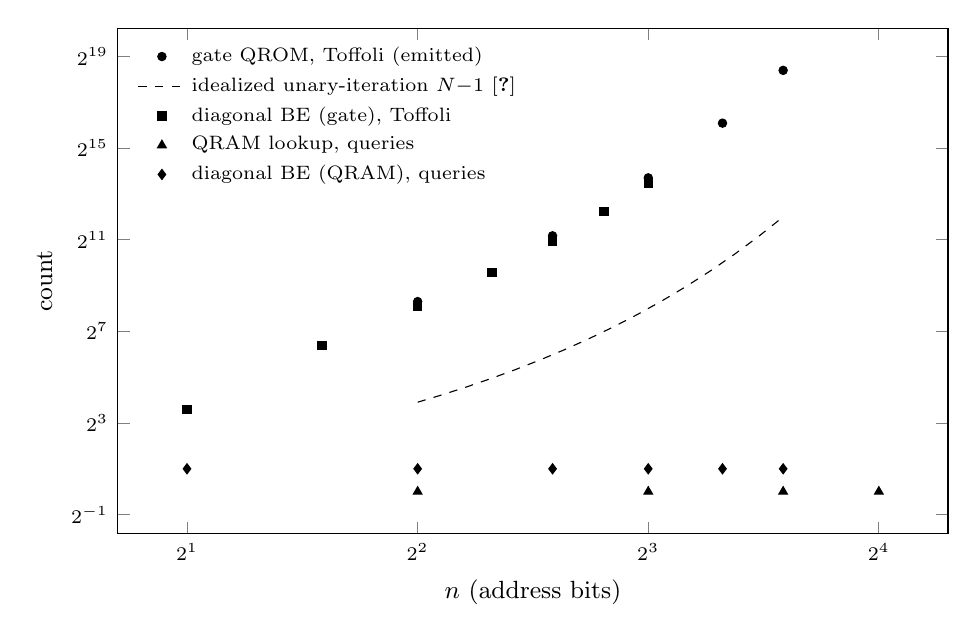
\begin{tikzpicture}
    \begin{loglogaxis}[
      width=\columnwidth, height=0.66\columnwidth,
      log basis x=2, log basis y=2,
      xlabel={$n$ (address bits)}, ylabel={count},
      xlabel style={font=\small}, ylabel style={font=\small},
      tick label style={font=\scriptsize},
      legend style={font=\scriptsize, draw=none, fill=none, at={(0.02,0.98)}, anchor=north west, inner sep=1pt},
      legend cell align=left,
    ]
      \addplot[only marks, mark=*, mark size=1.5pt] coordinates {(4,315) (6,2304) (8,13312) (10,69632) (12,344064)};
      \addlegendentry{gate QROM, Toffoli (emitted)}
      \addplot[domain=4:12, samples=16, dashed] {2^x - 1};
      \addlegendentry{idealized unary-iteration $N{-}1$ \cite{babbush2018encoding}}
      \addplot[only marks, mark=square*, mark size=1.5pt] coordinates {(2,12) (3,84) (4,270) (5,756) (6,1980) (7,4818) (8,11388)};
      \addlegendentry{diagonal BE (gate), Toffoli}
      \addplot[only marks, mark=triangle*, mark size=1.8pt] coordinates {(4,1) (8,1) (12,1) (16,1)};
      \addlegendentry{QRAM lookup, queries}
      \addplot[only marks, mark=diamond*, mark size=1.8pt] coordinates {(2,2) (4,2) (6,2) (8,2) (10,2) (12,2)};
      \addlegendentry{diagonal BE (QRAM), queries}
    \end{loglogaxis}
  \end{tikzpicture}
  \caption{QRAM as a first-class resource, measured.  Flat marks are query
  counts (independent of $n$); steep marks are gate-synthesized
  realizations of the same data access; the dashed line is the idealized
  unary-iteration QROM model.  The vertical separation---one query against
  $10^4$--$10^5$ Toffoli, and the $84\times$ gap between the idealized
  model and the emitted network at $n{=}12$---is the quantitative content
  of the access-model abstraction.}
  \label{fig:qram-queries}
\end{figure}

\begin{table*}[t]
  \centering
  \caption{QRAM query counts and gate-level costs across the solver stack:
  the fourteen closed input-model cases of \texttt{examples/input\_models.py}
  (same problem per family, different data paths), estimated on the
  exported RIR artifacts (\texttt{tools/build\_qram\_queries.py}).  Queries
  are broken down by resource role (a = angle database, t = coefficient
  table, f/i = forward/inverse grid banks).}
  \label{tab:solver-qram}
  \small
  \setlength{\tabcolsep}{4pt}\begin{tabular}{@{}llrrrrrl@{}}
    \toprule
    \tabhead{family} & \tabhead{input model (case)} & \tabhead{qubits} & \tabhead{Toffoli} & \tabhead{exact $T$} & \tabhead{rot.} & \tabhead{Q} & \tabhead{query breakdown} \\
    \midrule
    LCHS & given spectral & 10 & 728 & 55 & 58 & 0 & --- \\
    LCHS & spectral, QRAM prepare & 19 & 2\,036 & 95 & 258 & 40 & a40 \\
    LCHS & QRAM grid & 40 & 19\,632 & 179 & 242 & 84 & a4 f20 i20 t40 \\
    Carleman & stencil, gate & 20 & 3\,150 & 52 & 164 & 0 & --- \\
    Carleman & spectral ports & 21 & 14\,626 & 676 & 164 & 0 & --- \\
    Carleman & coefficient QRAM & 49 & 4\,245 & 88 & 362 & 36 & a12 t24 \\
    CBMD & given spectral & 11 & 1\,804 & 95 & 120 & 0 & --- \\
    CBMD & spectral, QRAM prepare & 20 & 4\,668 & 167 & 480 & 72 & a72 \\
    CBMD & QRAM grid & 41 & 44\,024 & 315 & 432 & 148 & a4 f36 i36 t72 \\
    CBMD & QHAM coefficient QRAM & 168 & 467\,750 & 2\,393 & 5\,621 & 352 & a28 t324 \\
    QHAM & stencil, gate & 151 & 68\,073 & 438 & 816 & 0 & --- \\
    QHAM & spectral ports & 152 & 224\,581 & 7\,054 & 896 & 0 & --- \\
    QHAM & coefficient, gate angles & 168 & 71\,343 & 510 & 1\,262 & 0 & --- \\
    QHAM & coefficient QRAM & 168 & 69\,658 & 538 & 1\,388 & 100 & a28 t72 \\
    \bottomrule
  \end{tabular}
\end{table*}

The estimates live at the logical level: rotation synthesis is accounted by
a leading-order model \cite{ross2016optimal}, and $T$ factories,
distillation, routing, and surface-code cycles are out of scope---the
physical layer of \cite{beverland2022assessing,gidney2025rsa} remains
future work, as does flowing these numbers back into per-module promise
attributes (R6).


\section{Glossary of recurring identifiers}
\label{app:glossary}

The code surface on which this paper relies is deliberately small---fifteen
names cover every program printed here, from the minimal Bell listing to
the QFVM pipeline.  Two conventions organize them.  First, the layering of
\figref{fig:stack} is visible in the prefixes: \texttt{Builder} and
\texttt{Operation} belong to the construction layer, unadorned names such
as \texttt{Module}, \texttt{Ref}, and \texttt{Load} are RIR concepts, and
the \texttt{abstract\_*} family lives in the algorithm libraries, which
declare what a solver \emph{needs} without constructing anything.
Second, solver entry points are uniform fronts rather than class
hierarchies: \texttt{linear\_qode} and \texttt{carleman\_qode} take the
family as data (a name string) together with injectable protocol
arguments, which is what allows the one-line family swaps shown in
\lstref{lst:qode-swap} and Appendix~\ref{app:families}.

\begin{table}[ht]
  \centering
  \caption{Recurring identifiers used throughout the paper.}
  \label{tab:glossary}
  \small
  \setlength{\tabcolsep}{4pt}\setlength{\tabcolsep}{4pt}\begin{tabular}{@{}p{3.3cm}p{10.4cm}@{}}
    \toprule
    \tabhead{Identifier} & \tabhead{Meaning} \\
    \midrule
    \texttt{Builder} & embedded module constructor over typed register views \\
    \texttt{Operation} & finished builder product; satisfies unitary / state-preparation / block-encoding protocols \\
    \texttt{Module} (RIR) & named typed interface + body (or absent body $=$ open oracle slot) \\
    \texttt{Ref} / \texttt{Span} & declarative register view; $(\text{register}, \text{start}, \text{width})$ \\
    \texttt{QRAM} & typed resource: address width, data width, runtime table binding \\
    \texttt{Load} & reversible memory access $|a\rangle|d\rangle \mapsto |a\rangle|d \oplus M[a]\rangle$ \\
    \texttt{bind} / \texttt{unresolved} & oracle linking pass / open-slot gap analysis \\
    \texttt{BlockEncoding} & operation + normalization $\alpha$ + capabilities \\
    \texttt{QODEProblem} & linear ODE input object (generator BE, initial state, promises) \\
    \texttt{linear\_qode} & uniform entry over LCHS / Schr\"odingerization / CBMD with injectable Hamiltonian-function kernel \\
    \texttt{carleman\_qode} & nonlinear path: polynomial ODE $\rightarrow$ cutoff-$K$ lift $\rightarrow$ any linear solver \\
    \texttt{qram\_coefficient\_}\\ \texttt{encoding} & coefficient diagonal as an open angle database, bound to a gate or QRAM realization \\
    \texttt{make\_costa\_qlss} /\\ \texttt{make\_cks\_qlss} & the two QLSS kernels (interchangeable) \\
    \texttt{SpectralPromise} & norm / smallest-singular-value bounds with provenance \\
    \texttt{compile\_function} & pure-Python function $\rightarrow$ SSA MIR $\rightarrow$ reversible RIR module \\
    \texttt{quantikz} & circuit-diagram export; calls as named boxes, open slots dashed \\
    \texttt{export\_originir} & modular textual export (module calls preserved) \\
    \bottomrule
  \end{tabular}
\end{table}

The table doubles as a stability statement: these names constitute the
public surface of \pqlang{} 0.8.0 on which every doctest, gallery case,
and catalog entry of Appendix~\ref{app:repro} is pinned.  Readers who want
the next level of detail---constructor signatures, protocol definitions,
and the per-family configuration records---will find them in the API
reference shipped with the distribution, which is generated from the same
docstrings the examples exercise.
